\documentclass[12pt,letterpaper]{article}
\usepackage{graphicx,textcomp}
\usepackage{natbib}
\usepackage{setspace}
\usepackage{fullpage}
\usepackage{color}
\usepackage[reqno]{amsmath}
\usepackage{amsthm}
\usepackage{fancyvrb}
\usepackage{amssymb,enumerate}
\usepackage[all]{xy}
\usepackage{endnotes}
\usepackage{lscape}
\newtheorem{com}{Comment}
\usepackage{float}
\usepackage{hyperref}
\newtheorem{lem} {Lemma}
\newtheorem{prop}{Proposition}
\newtheorem{thm}{Theorem}
\newtheorem{defn}{Definition}
\newtheorem{cor}{Corollary}
\newtheorem{obs}{Observation}
\usepackage[compact]{titlesec}
\usepackage{dcolumn}
\usepackage{tikz}
\usetikzlibrary{arrows}
\usepackage{multirow}
\usepackage{xcolor}
\newcolumntype{.}{D{.}{.}{-1}}
\newcolumntype{d}[1]{D{.}{.}{#1}}
\definecolor{light-gray}{gray}{0.65}
\usepackage{url}
\usepackage{listings}
\usepackage{color}

\definecolor{codegreen}{rgb}{0,0.6,0}
\definecolor{codegray}{rgb}{0.5,0.5,0.5}
\definecolor{codepurple}{rgb}{0.58,0,0.82}
\definecolor{backcolour}{rgb}{0.95,0.95,0.92}

\lstdefinestyle{mystyle}{
	backgroundcolor=\color{backcolour},   
	commentstyle=\color{codegreen},
	keywordstyle=\color{magenta},
	numberstyle=\tiny\color{codegray},
	stringstyle=\color{codepurple},
	basicstyle=\footnotesize,
	breakatwhitespace=false,         
	breaklines=true,                 
	captionpos=b,                    
	keepspaces=true,                 
	numbers=left,                    
	numbersep=5pt,                  
	showspaces=false,                
	showstringspaces=false,
	showtabs=false,                  
	tabsize=2
}
\lstset{style=mystyle}
\newcommand{\Sref}[1]{Section~\ref{#1}}
\newtheorem{hyp}{Hypothesis}

\title{Problem Set 1}
\date{Due: October 3, 2021}
\author{Applied Stats/Quant Methods 1}

\begin{document}
	\maketitle
	
	\section*{Instructions}
	\begin{itemize}
		\item Please show your work! You may lose points by simply writing in the answer. If the problem requires you to execute commands in \texttt{R}, please include the code you used to get your answers. Please also include the \texttt{.R} file that contains your code. If you are not sure if work needs to be shown for a particular problem, please ask.
		\item Your homework should be submitted electronically on GitHub in \texttt{.pdf} form.
		\item This problem set is due before 8:00 on Friday October 3, 2021. No late assignments will be accepted.
		\item Total available points for this homework is 100.
	\end{itemize}
	
	\vspace{1cm}
	\section*{Question 1 (50 points): Education}
	
	A school counselor was curious about the average of IQ of the students in her school and took a random sample of 25 students' IQ scores. The following is the data set:\\
	\vspace{.5cm}
	

	
	\vspace{1cm}
	
	\begin{enumerate}
		\item Find a 90\% confidence interval for the average student IQ in the school.\\

\begin{verbatim}
	First I calculate the average IQ for the sample
\end{verbatim}
\lstinputlisting[language=R, firstline=10, lastline=10]{PS01.R}  
\begin{verbatim}
Then I calculate the standard deviation in the sample
\end{verbatim}		
\lstinputlisting[language=R, firstline=13, lastline=13]{PS01.R}  
\begin{verbatim}
Next I calculate the margin of error using the standard deviation and sample size.
\end{verbatim}	
\lstinputlisting[language=R, firstline=18, lastline=18]{PS01.R}  
\begin{verbatim}
Finally, I calculate the upper and lower intervals
\end{verbatim}	
\lstinputlisting[language=R, firstline=21, lastline=25]{PS01.R}  


		\item Next, the school counselor was curious  whether  the average student IQ in her school is higher than the average IQ score (100) among all the schools in the country.\\ 
		


		\noindent Using the same sample, conduct the appropriate hypothesis test with $\alpha=0.05$.
	\end{enumerate}

\begin{verbatim}
I conduct a one sample t-test
\end{verbatim}
\lstinputlisting[language=R, firstline=29, lastline=30]{PS01.R}  
\begin{verbatim}
Because p>0.05, we do not have evidence to reject the null-hypothesis, that the
average student IQ in the school is the same or lower than the average IQ score
(100) among all the schools in the country.

Alternatively, we can calculate this manually:
\end{verbatim}
\lstinputlisting[language=R, firstline=36, lastline=39]{PS01.R}

	\newpage
	
	\section*{Question 2 (50 points): Political Economy}
	
	\noindent Researchers are curious about what affects the amount of money communities spend on addressing homelessness. The following variables constitute our data set about social welfare expenditures in the USA. \\
	\vspace{.5cm}
	
	
	\begin{tabular}{r|l}
		\texttt{State} &\emph{50 states in US} \\
		\texttt{Y} & \emph{per capita expenditure on shelters/housing assistance in state}\\
		\texttt{X1} &\emph{per capita personal income in state} \\
		\texttt{X2} &  \emph{Number of residents per 100,000 that are "financially insecure" in state}\\
		\texttt{X3} &  \emph{Number of people per thousand residing in urban areas in state} \\
		\texttt{Region} &  \emph{1=Northeast, 2= North Central, 3= South, 4=West} \\
	\end{tabular}
	
	\vspace{.5cm}
	\noindent Explore the \texttt{expenditure} data set and import data into \texttt{R}.
	\vspace{.5cm}
	\lstinputlisting[language=R, firstline=54, lastline=54]{PS01.R}  
	\vspace{.5cm}
	\begin{itemize}
		
		\item
		Please plot the relationships among \emph{Y}, \emph{X1}, \emph{X2}, and \emph{X3}? What are the correlations among them (you just need to describe the graph and the relationships among them)?
		\vspace{.5cm}
		\item
\lstinputlisting[language=R, firstline=45, lastline=45]{PS01.R} 
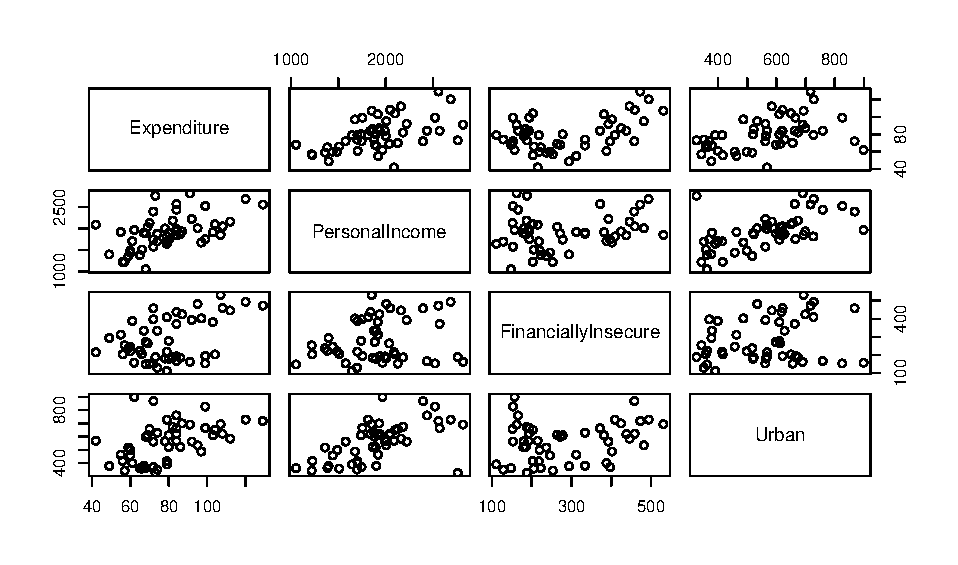
\includegraphics[width=.75\textwidth]{pairs_plot}
\begin{verbatim}
Each of the three independent variables is positively associated with
Expenditure on Shelters/Housing Assistance. Personal income and
urban population appear to have a strong positive correlation.
On the other hand, Financial Insecurity doesn't appear to have a
strong association with either Urban population or Personal Income.
\end{verbatim}






		Please plot the relationship between \emph{Y} and \emph{Region}? On average, which region has the highest per capita expenditure on housing assistance?
		\vspace{.5cm}
		\item
\begin{verbatim}
I produce a boxplot in order to compare the average expenditure on
shelters/housing assistance across the 4 regions.
\end{verbatim}

\lstinputlisting[language=R, firstline=60, lastline=60]{PS01.R}
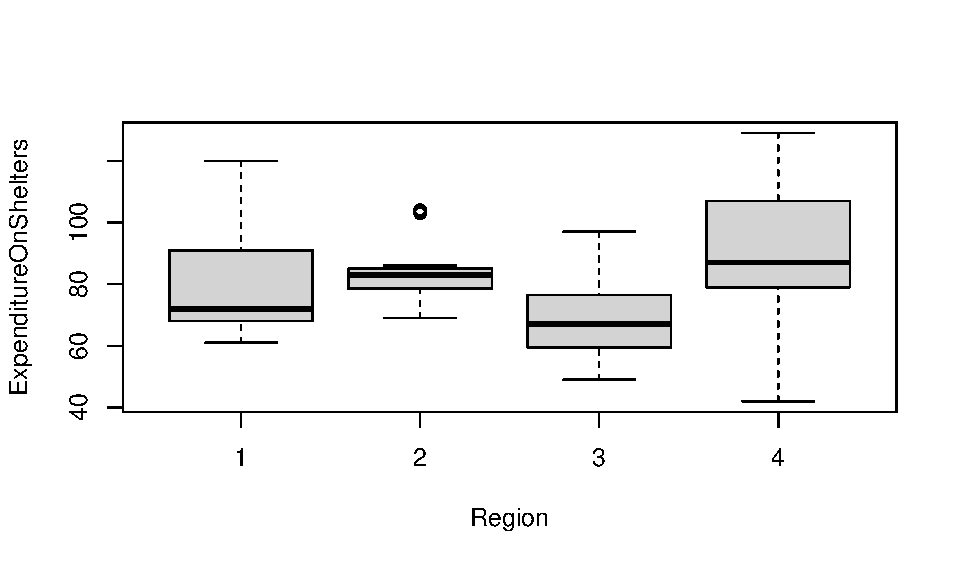
\includegraphics[width=.75\textwidth]{boxplot_regions}
\begin{verbatim}
This box plot shows that expenditure on shelters/housing assistance is
highest in the Western region of the US.
\end{verbatim}

		Please plot the relationship between \emph{Y} and \emph{X1}? Describe this graph and the relationship. Reproduce the above graph including one more variable \emph{Region} and display different regions with different types of symbols and colors.

\begin{verbatim}
I produce a scatterplot of Expenditure on Shelters vs Personal Income,
with different regions in different colours:
\end{verbatim}

\lstinputlisting[language=R, firstline=68, lastline=69]{PS01.R} 
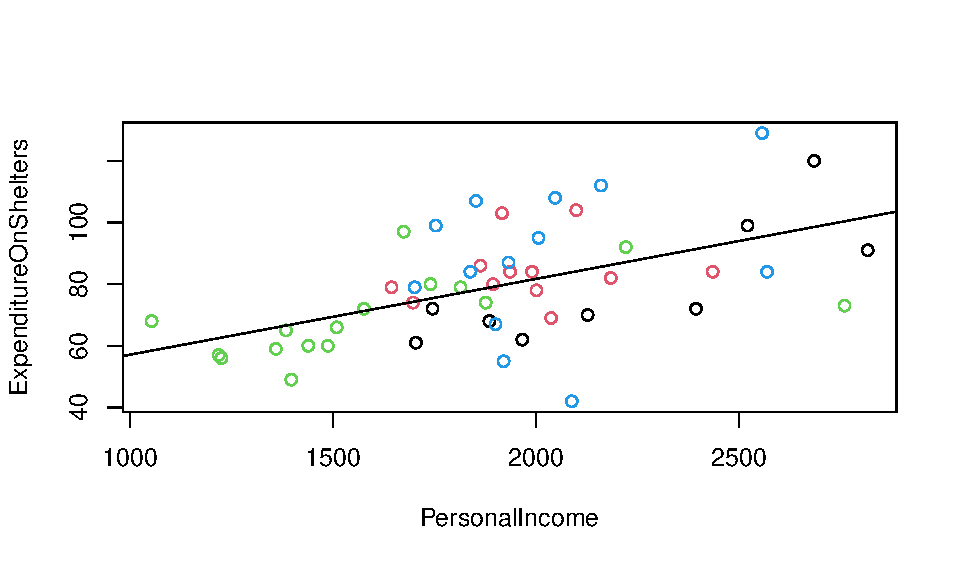
\includegraphics[width=.75\textwidth]{scatterplot_regions_coloured}

\begin{verbatim}
to better understand the data and see how states in different regions differ,
I add 4 lines of best fit, one for each of the 4 regions:
\end{verbatim}
\lstinputlisting[language=R, firstline=74, lastline=82]{PS01.R} 
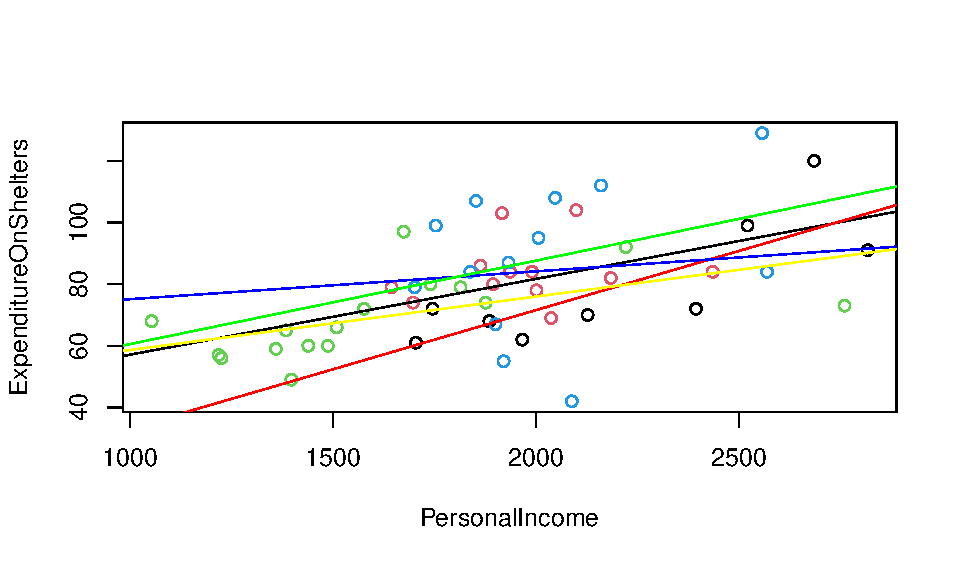
\includegraphics[width=.75\textwidth]{scatterplot_with_lines}
\begin{verbatim}
It appears from the data that the positive association between Personal
Income and higher rates of expenditure on shelters and housing assistance
is most significant in the Northeast, and is least significant in the
Northcentral region, with the other two regions falling in betweeen.
Northeast states also appear to have the highest Personal Incomes
overall, whilst southern states have the lowest incomes.
\end{verbatim}
	\end{itemize}
	
	
\end{document}